% radiosynth - From MHD to MHz: gyroresonance emission step by step, with a simple code
% Copyright (C) 2026 Soumitra Hazra
% Compile with: pdflatex gyroresonance_simple.tex (twice);
% needs side_view.pdf, gyroresonance_simple_fig.pdf and gyroresonance_simple.py
\documentclass[11pt,a4paper]{article}
\usepackage[T1]{fontenc}
\usepackage{lmodern}
\usepackage[margin=2.5cm]{geometry}
\usepackage{amsmath,amssymb,bm}
\usepackage{booktabs}
\usepackage{graphicx}
\usepackage{xcolor}
\usepackage{enumitem}
\usepackage{needspace}
\usepackage{listings}
\usepackage[font=small,labelfont=bf]{caption}
\usepackage[colorlinks=true,linkcolor=blue!50!black,urlcolor=blue!50!black]{hyperref}

\definecolor{accent}{RGB}{31,78,121}
\definecolor{boxbg}{RGB}{236,243,250}
\definecolor{codebg}{RGB}{247,247,247}
\newcommand{\code}[1]{\texttt{#1}}
\newcommand{\vect}[1]{\bm{#1}}
\newcommand{\dd}{\mathrm{d}}
\newcommand{\kB}{k_\mathrm{B}}
\newcommand{\nuB}{\nu_B}
\setlength{\parskip}{5pt}
\setlength{\parindent}{0pt}
\setlength{\emergencystretch}{2.5em}
\setlist{itemsep=2pt,topsep=3pt}

\lstset{language=Python, basicstyle=\ttfamily\footnotesize, backgroundcolor=\color{codebg},
  frame=single, rulecolor=\color{gray!40}, framesep=4pt, xleftmargin=6pt, xrightmargin=6pt,
  keywordstyle=\color{accent}\bfseries, commentstyle=\color{green!40!black}\itshape,
  stringstyle=\color{red!50!black}, showstringspaces=false, columns=fullflexible,
  breaklines=true, upquote=true, literate={–}{{--}}1 {—}{{---}}1}

\newcommand{\stephead}[2]{\needspace{8\baselineskip}\vspace{8pt}{\Large\bfseries\color{accent} #1\par}\vspace{1pt}{\itshape\color{gray} #2\par}\vspace{3pt}}
\newcommand{\remember}[1]{\par\smallskip\noindent\colorbox{boxbg}{\parbox{\dimexpr\linewidth-2\fboxsep}{\small\textbf{Remember:} #1}}\par\smallskip}

\hypersetup{pdftitle={Gyroresonance emission, step by step},pdfauthor={Soumitra Hazra}}

\begin{document}

\begin{center}
{\LARGE\bfseries\color{accent} Gyroresonance emission, step by step\par}
\vspace{0.25cm}
{\large with a simple Python code that anyone can read\par}
\vspace{0.4cm}
{\normalsize Soumitra Hazra\par}
{\small Companion to \textsf{radiosynth} 2.2.0 --- \emph{From MHD to MHz} --- \url{https://github.com/soumitrahazra/radiosynth}\par}
\end{center}

\vspace{0.2cm}
This note explains how to compute the thermal gyroresonance radio emission of a sunspot, one
step at a time, and gives a short Python program, \code{gyroresonance\_simple.py}, that does
exactly these steps and nothing else. The program needs only \code{numpy} and
\code{matplotlib}; it is about 300 lines long, most of them comments, and it runs in about half
a minute:
\begin{lstlisting}
python gyroresonance_simple.py      # writes gyroresonance_simple_fig.png
\end{lstlisting}
Each section below is one \code{STEP} of the program: first the idea, then the equation, then
the lines of code that compute it. The full program is printed in the Appendix. It uses the
same physics as \textsf{radiosynth} and gives the same images to 0.01\,\% (see \emph{Check against radiosynth}),
but it is written for reading, not for speed or generality: the model is a flat box seen
straight from above.

%======================================================================
\stephead{The plan}{Seven steps from a magnetic field to a radio image}

\begin{enumerate}[label=\textbf{\arabic*.},start=0]
\item Constants.
\item A model of an active region: density, temperature and magnetic field in a box.
\item One straight line of sight per pixel.
\item The plasma along each line: field strength, angle to the line of sight, gyrofrequency.
\item The ordinary (free--free) absorption of the two wave modes.
\item The gyroresonance layers crossed by each line, and how opaque they are.
\item The radiative transfer: add up the light along each line, for right- and left-handed waves.
\item What the telescope sees: brightness temperature, circular polarisation and flux.
\end{enumerate}

%======================================================================
\stephead{STEP 0.\quad Constants}{Everything in cgs units}

We use cgs units, like most solar radio papers. Two combinations appear again and again:
\begin{equation}
  \nuB=\frac{eB}{2\pi m_ec}=2.80\times10^{6}\ \text{Hz}\times\frac{B}{1\,\text{G}},
  \qquad
  \frac{\pi e^2}{m_ec}=0.02654\ \text{cm}^2\,\text{s}^{-1}.
\end{equation}
The first is the \emph{gyrofrequency}: how many times per second an electron goes around a field
line. The second sets the strength of the absorption.
\begin{lstlisting}
NU_B_PER_GAUSS = E / (2.0 * math.pi * ME * C)     # 2.80e6 Hz per gauss
GR_PREFACTOR   = math.pi * E**2 / (ME * C)        # 0.02654 cm^2/s
\end{lstlisting}

%======================================================================
\stephead{STEP 1.\quad The model}{A box above two sunspots}

The box is 140\,Mm wide and 150\,Mm high; $x$, $y$ are horizontal and $z$ is the height above
the photosphere, all in Mm.

\textbf{Density} falls off exponentially with height, and the \textbf{temperature} is the same
everywhere (to keep things simple):
\begin{equation}
  n_e(z)=n_0\,e^{-z/H},\quad n_0=2\times10^9\ \text{cm}^{-3},\ H=35\ \text{Mm};\qquad
  T_e=2.5\ \text{MK}.
\end{equation}

\textbf{The magnetic field} is that of a small bar magnet (a dipole $\vect m$, pointing along $x$)
buried 35\,Mm below the surface. Its two ends make two spots of opposite polarity:
\begin{equation}
  \vect B(\vect r)=\frac{3(\vect m\cdot\vect r)\,\vect r-\vect m\,r^2}{r^5},
\end{equation}
with $\vect r$ measured from the dipole, scaled so that $|\vect B|=2500$\,G at the surface right above
it. Fig.~\ref{fig:side} shows the field: strongest near the surface, weakening with height.

\begin{lstlisting}
def density(z):
    return N0 * np.exp(-z / H_N)

def magnetic_field(x, y, z):
    rx, ry, rz = x, y, z + DEPTH            # position relative to the dipole
    r2 = rx**2 + ry**2 + rz**2
    r5 = r2**2.5
    mdotr = mx * rx
    bx = (3.0 * mdotr * rx - mx * r2) / r5
    by = (3.0 * mdotr * ry) / r5
    bz = (3.0 * mdotr * rz) / r5
    ...                                     # scaled to B_MAX
\end{lstlisting}

\begin{figure}[ht]
\centering
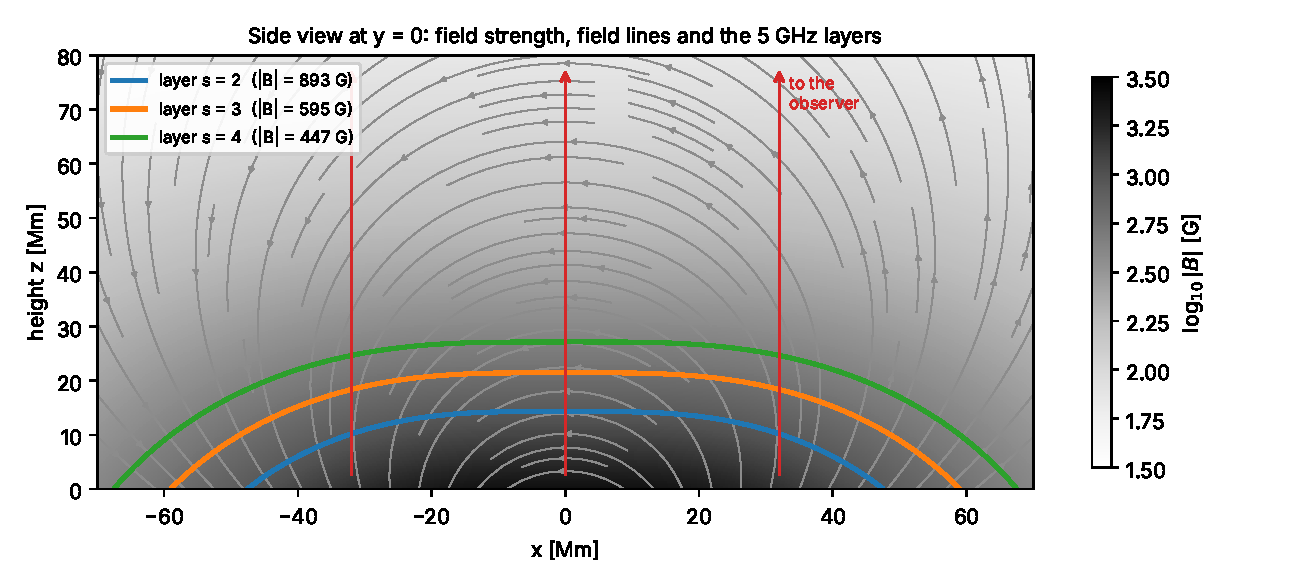
\includegraphics[width=\textwidth]{side_view.pdf}
\caption{Side view of the model ($y=0$): field strength (grey), field lines, and the three surfaces
where gyroresonance happens at 5\,GHz (Step~5). The red arrows are three lines of sight, looking
straight down at the spots ($x=\pm32$\,Mm) and between them ($x=0$).}
\label{fig:side}
\end{figure}

\remember{any MHD model can replace these three functions; \textsf{radiosynth} does exactly that
with the density, temperature and field of BATS-R-US, PLUTO or other simulations.}

%======================================================================
\stephead{STEP 2.\quad The lines of sight}{One straight line per pixel, looking down}

We look straight down from above: one vertical line per pixel, $100\times100$ pixels. The wave
travels \emph{up}, towards us, so the direction towards the observer is
\begin{equation}
  \hat{\vect k}=(0,0,1).
\end{equation}
At microwave frequencies the plasma is far too thin to bend the rays, so straight lines are
fine. Each line is sampled at 601 heights from the top ($z=150$\,Mm, point 0, nearest to us)
down to the photosphere, every 0.25\,Mm.
\begin{lstlisting}
c = -0.5 * FOV + (np.arange(NPIX) + 0.5) * FOV / NPIX    # pixel centres
X, Y = np.meshgrid(c, c)
z = np.linspace(Z_TOP, 0.0, NZ + 1)                      # top -> photosphere
\end{lstlisting}

%======================================================================
\stephead{STEP 3.\quad The plasma along each line}{What every sample point needs}

At each point we need the field strength $B=|\vect B|$, the angle $\theta$ between the field and the
line of sight, and three frequencies compared with the observing frequency $\nu$:
\begin{equation}
  \cos\theta=\frac{\vect B\cdot\hat{\vect k}}{B}=\frac{B_z}{B},\qquad
  \nuB=2.80\,\text{MHz}\times B,\qquad
  X=\frac{\nu_p^2}{\nu^2},\quad \nu_p^2=\frac{e^2n_e}{\pi m_e},\qquad
  Y=\frac{\nuB}{\nu}.
\end{equation}
$\nu_p$ is the plasma frequency. $X$ tells how dense the plasma is for this wave (it can only
travel where $X$ is small enough), and $Y$ how strong the field is ($Y=1/s$ exactly on the $s$-th
layer).
\begin{lstlisting}
cos_theta = bz / b                     # angle between B and k = (0, 0, 1)
nu_b = NU_B_PER_GAUSS * b              # gyrofrequency [Hz]
nu_p2 = E**2 * ne / (math.pi * ME)     # plasma frequency squared
Xmi = nu_p2 / freq**2                  # X
Ymi = nu_b / freq                      # Y
\end{lstlisting}

%======================================================================
\stephead{STEP 4.\quad Free--free absorption of the two modes}{The ``background'' opacity}

In a magnetic field a radio wave can only travel in two ways, the two \emph{modes}: the
\textbf{x-mode} (extraordinary), whose electric field rotates with the gyrating electrons, and
the \textbf{o-mode} (ordinary). Even without gyroresonance, the ordinary collisions of electrons
with ions absorb the waves (free--free absorption, Dulk 1985):
\begin{equation}
  \kappa_\text{ff}=9.78\times10^{-3}\,\frac{n_e^2}{\nu^2T_e^{3/2}}\,
  \big(24.5+\ln T_e-\ln\nu\big)\ \ \text{cm}^{-1},
\end{equation}
slightly more for the x-mode and less for the o-mode:
\begin{equation}
  \kappa_x=\frac{\kappa_\text{ff}}{(1-q)^2},\qquad \kappa_o=\frac{\kappa_\text{ff}}{(1+q)^2},\qquad
  q=Y|\cos\theta|\ (\le0.9).
\end{equation}
For each step between two sample points (length $\Delta\ell$) the optical depth is
$\Delta\tau_\text{ff}=\kappa\,\Delta\ell$, with $\kappa$ taken at the middle of the step.
\begin{lstlisting}
kappa = 9.78e-3 * ne**2 / (freq**2 * te**1.5) * G
q = np.minimum(Ymi * np.abs(cos_theta), 0.9)
kappa_x, kappa_o = kappa / (1 - q)**2, kappa / (1 + q)**2
dtau_x, dtau_o = kappa_x * dl, kappa_o * dl
\end{lstlisting}
For our model this alone gives at most $0.23$\,MK at 5\,GHz --- far too faint to explain a
sunspot. The next step adds what is missing.

%======================================================================
\stephead{STEP 5.\quad The gyroresonance layers}{The heart of the calculation}

\textbf{(a) Where.} Electrons spiralling in the field absorb and emit at their gyrofrequency
and its multiples. A wave of frequency $\nu$ is affected only where
\begin{equation}
  \nu=s\,\nuB,\qquad s=1,2,3,\ldots\qquad\Longleftrightarrow\qquad
  B=B_s=\frac{\nu}{s\times2.80\,\text{MHz/G}} .
\end{equation}
These are thin surfaces of constant field strength, the \emph{layers}. At 5\,GHz they are at
$B_2=893$\,G, $B_3=595$\,G, $B_4=447$\,G (coloured lines in Fig.~\ref{fig:side}).

\textbf{(b) Finding them along a line.} Between two neighbouring points $k$ and $k+1$ there is
a layer of harmonic $s$ if $s\nuB-\nu$ changes sign:
\begin{equation}
  (s\,\nu_{B,k}-\nu)(s\,\nu_{B,k+1}-\nu)<0 .
\end{equation}
Where exactly? By linear interpolation, at the fraction
$u=(\nu/s-\nu_{B,k})/(\nu_{B,k+1}-\nu_{B,k})$ of the step, and we take $n_e$, $T_e$, $\cos\theta$ and $X$
there.

\textbf{(c) How thick.} The layer is thin, and its strength depends on how fast $B$ changes
along the line, measured by the \emph{magnetic scale length}
\begin{equation}
  L_B=\left|\frac{B}{\dd B/\dd\ell}\right|\ \approx\ \frac{B_s\,\Delta\ell}{|B_{k+1}-B_k|}.
\end{equation}

\textbf{(d) How opaque.} The optical depth of the layer is
\begin{equation}
  \boxed{\;
  \tau_s=\frac{\pi e^2}{m_ec}\,\frac{n_e\,L_B}{\nu}\;\frac{s^2}{s!}
   \left(\frac{s^2\beta_T^2\sin^2\theta}{2}\right)^{s-1}F(\theta),\qquad
   \beta_T^2=\frac{\kB T_e}{m_ec^2}\;}
\end{equation}
($\beta_T^2\approx4\times10^{-4}$ at 2.5\,MK). The bracket raised to the power $s-1$ makes each higher
harmonic several hundred times weaker, so only $s=2$, 3 and sometimes 4 matter. The factor
$\sin^2\theta$ makes a layer seen \emph{along} the field almost transparent.

\textbf{(e) Which mode.} $F$ says how well each mode couples to the electrons:
\begin{equation}
  F_x=\frac{(1+|T||\cos\theta|)^2}{1+T^2},\qquad F_o=\frac{(|T|-|\cos\theta|)^2}{1+T^2},
\end{equation}
where $|T|$ measures how circular the x-mode is (1: circular, 0: linear),
\begin{equation}
  |T|=\frac{2(1-X)|\cos\theta|}{Y\sin^2\theta+\sqrt{Y^2\sin^4\theta+4(1-X)^2\cos^2\theta}},
\end{equation}
with $Y=1/s$. Along the field $F_x=2$ and $F_o=0$: the x-mode, rotating with the electrons, is
absorbed far more. (On the $s=1$ layer the x-mode cannot exist at all, so its $\tau$ is set to 0.)

\begin{lstlisting}
crosses = (s * f0 - freq) * (s * f1 - freq) < 0          # (b) a layer in this step?
u = (freq / s - f0) / (f1 - f0)                         #     where in the step
ne_c, te_c, cos_c, X_c = at(ne), at(te), at(cos_theta), at(Xmi)
b_s = freq / (s * NU_B_PER_GAUSS)                       # (a) |B| on the layer
l_b = b_s * dl / np.abs(b[..., 1:] - b[..., :-1])       # (c) L_B
beta2 = KB * te / (ME * C**2)                           # (d) tau_s
tau = (GR_PREFACTOR * ne * l_b / freq * s**2 / math.factorial(s)
       * (0.5 * s**2 * beta2 * sin2)**(s - 1) * F)      # F from (e)
\end{lstlisting}
The layer optical depths of a step are added to its free--free optical depth, for each mode.

\remember{at each frequency, the emission comes from a few thin layers of constant $|B|$; the x-mode
sees them as opaque walls, the o-mode as much thinner veils.}

%======================================================================
\stephead{STEP 6.\quad Adding up the light}{Radiative transfer, from the observer inwards}

\textbf{How bright each step glows.} The electrons are thermal, so each mode glows exactly as
much as it absorbs (Kirchhoff's law), at the temperature of the gas. It is easiest to count
everything in temperature units: for one polarisation, the ``brightness temperature''
$T_p=I_pc^2/(\kB\nu^2)$. A step whose optical depth comes from several parts (free--free and maybe
a layer) glows at their optical-depth-weighted temperature
\begin{equation}
  T_\text{step}=\frac{\sum_i\tau_iT_i}{\sum_i\tau_i}
\end{equation}
(just $T_e$ in our isothermal model).

\textbf{Walking along the line.} Starting at the observer, each step adds its glow, dimmed by
everything in front of it:
\begin{equation}
  \boxed{\;T_p\ \leftarrow\ T_p+T_\text{step}\left(1-e^{-\Delta\tau}\right)e^{-\tau},\qquad
  \tau\ \leftarrow\ \tau+\Delta\tau\;}
\end{equation}
A transparent step ($\Delta\tau\ll1$) adds little; an opaque one adds its full temperature, but only
if the gas in front ($\tau$) has not already hidden it. Behind an opaque layer, nothing more is
seen.

\textbf{Right- and left-handed light.} A telescope measures right-hand ($R$) and left-hand ($L$)
circular polarisation. Where the field points towards us ($\cos\theta>0$), the x-mode is
right-handed; where it points away, left-handed. So in each step $R$ uses the x-mode optical depth
if $\cos\theta>0$ and the o-mode one otherwise, and $L$ the opposite. Finally, a wave stops where its
mode cannot exist (o-mode: $X\ge1$; x-mode: $X\ge1-Y$).
\begin{lstlisting}
pos = mid(cos_theta) > 0                          # field towards us?
dtau_R = np.where(pos, dtau_x, dtau_o)            # R: x-mode there, else o-mode
dtau_L = np.where(pos, dtau_o, dtau_x)
for k in range(nk):                               # walk along the line
    d = dtau[..., k]
    t_step = tT[..., k] / d
    t_pol += t_step * (1 - np.exp(-d)) * np.exp(-tau)
    tau += d
\end{lstlisting}

%======================================================================
\stephead{STEP 7.\quad What the telescope sees}{Brightness, polarisation, flux}

Each polarisation carries half of the light, so the brightness temperature of the total light
(Stokes $I$) and of the circular polarisation (Stokes $V$) are
\begin{equation}
  T_b=\tfrac12\,(T_R+T_L),\qquad T_V=\tfrac12\,(T_R-T_L),\qquad \frac{V}{I}=\frac{T_R-T_L}{T_R+T_L}.
\end{equation}
The flux density at the Earth, adding all pixels of solid angle $\Delta\Omega$
($=(\text{pixel size}/1\,\text{AU})^2$), is
\begin{equation}
  F=\frac{2\kB\nu^2}{c^2}\sum_\text{pixels}T_b\,\Delta\Omega,\qquad 1\ \text{sfu}=10^{-19}\ \text{erg\,s}^{-1}\text{cm}^{-2}\text{Hz}^{-1}.
\end{equation}
\begin{lstlisting}
tb = 0.5 * (t_R + t_L)
tb_v = 0.5 * (t_R - t_L)
pol = tb_v / tb
flux = 2 * KB * freq**2 / C**2 * tb.sum() * d_omega / 1e-19     # sfu
\end{lstlisting}

\begin{figure}[ht]
\centering
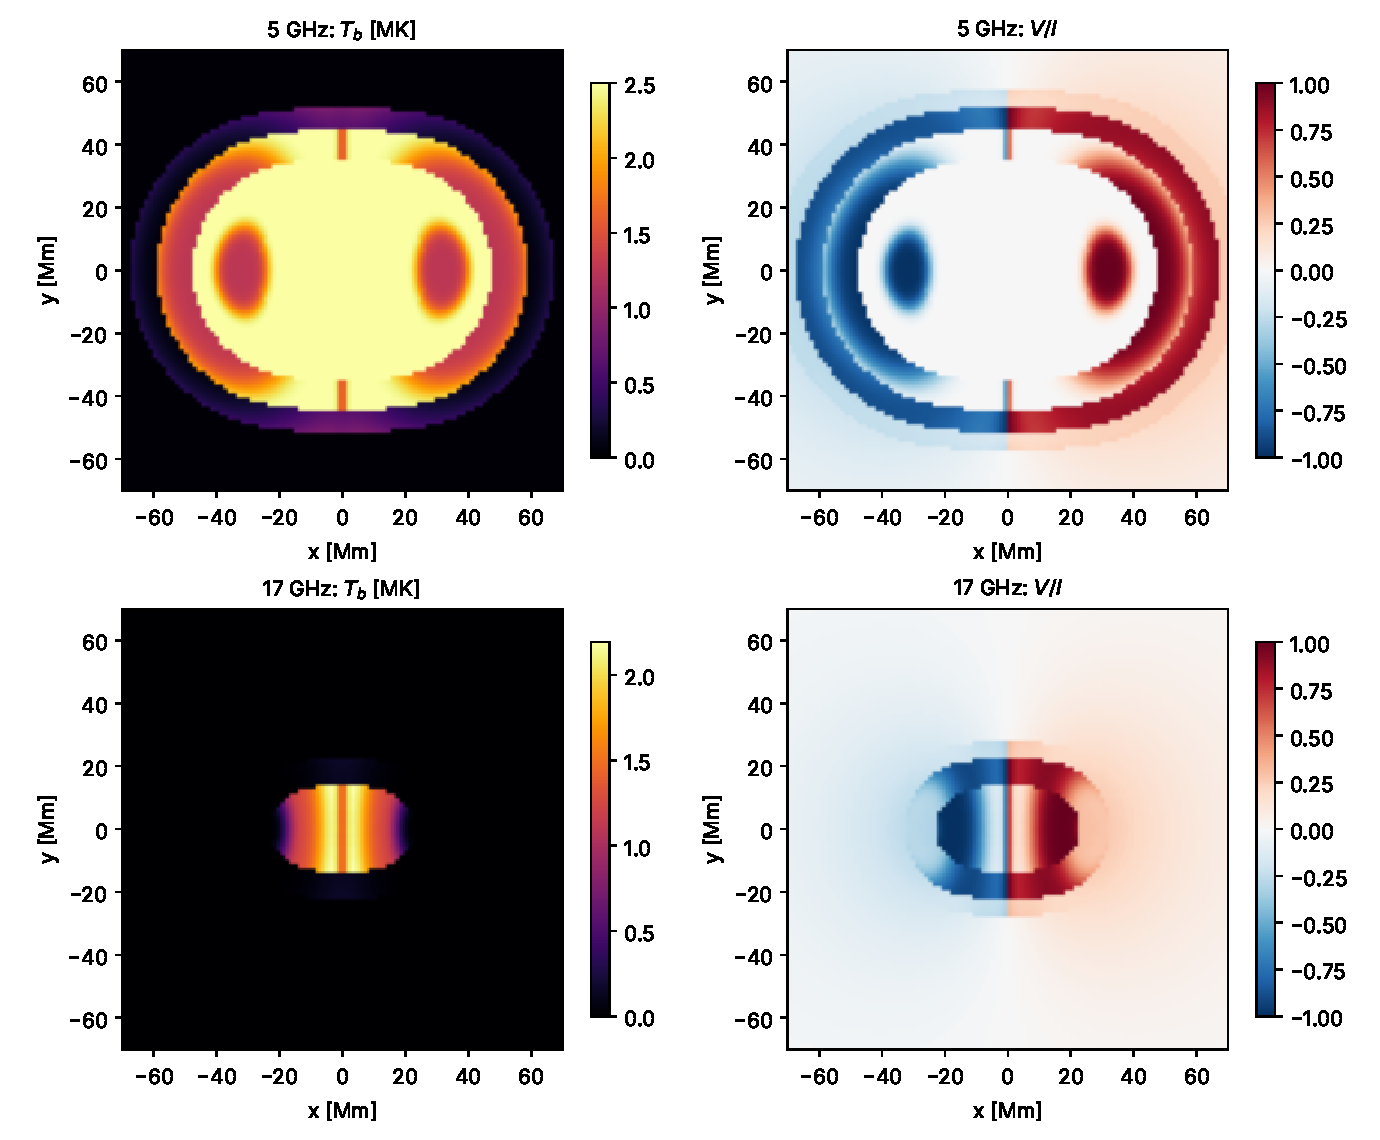
\includegraphics[width=0.86\textwidth]{gyroresonance_simple_fig.pdf}
\caption{The output of \code{gyroresonance\_simple.py}: brightness temperature and circular
polarisation $V/I$ at 5\,GHz (top) and 17\,GHz (bottom), seen from above.}
\label{fig:result}
\end{figure}

\textbf{Reading the result} (Fig.~\ref{fig:result}):
\begin{itemize}
\item \textbf{At 5\,GHz most of the region is at $T_b=2.5$\,MK $=T_e$}: every line crosses the $s=2$
      or $s=3$ layer, which is opaque in both modes (for example $\tau_R\approx1.7\times10^4$,
      $\tau_L\approx130$ at $x=y=15$\,Mm), so we see the temperature of the corona and no
      polarisation. The total flux is 68\,sfu, against 2.6\,sfu from free--free alone.
\item \textbf{The ring at the edge} is the $s=3$ and $s=4$ layers seen where they are only
      partly opaque, and mostly in the x-mode, hence strongly polarised.
\item \textbf{The spot centres ($x=\pm32$\,Mm) are darker and almost 100\,\% polarised.} There the
      field points straight up or down, along the line of sight: $\sin\theta\to0$, the layers become
      thin, and only the x-mode is still opaque ($\tau_R=29$, $\tau_L=0.006$). So $T_R=2.5$\,MK,
      $T_L\approx0$, $T_b=1.26$\,MK and $V/I=+0.99$ over the spot whose field points towards us, $-0.99$
      over the other. The total $V$ of the symmetric pair is zero.
\item \textbf{At 17\,GHz the source shrinks} to the core where $B>B_3=2024$\,G, close to the
      surface between the spots; the peak is 2.2\,MK and the flux 62\,sfu.
\end{itemize}

%======================================================================
\stephead{Check against radiosynth}{Same answer, to 0.01\,\%}\label{sec:check}

The script \code{check\_with\_radiosynth.py} (next to the program) puts the same model on a
\textsf{radiosynth} grid and computes the image with \code{rs.make\_gr\_image}, looking from above
with parallel rays. A low-resolution version runs with the tests of the package
(\code{tests/test\_simple\_gyroresonance.py}), so the two codes cannot drift apart unnoticed.
At full resolution:

\begin{center}
\small
\begin{tabular}{@{}l cc cc@{}}
\toprule
 & \multicolumn{2}{c}{5 GHz} & \multicolumn{2}{c}{17 GHz} \\
\cmidrule(lr){2-3}\cmidrule(lr){4-5}
 & simple code & radiosynth & simple code & radiosynth \\
\midrule
max $T_b$ [MK] & 2.500 & 2.500 & 2.195 & 2.200 \\
flux [sfu] & 67.88 & 67.88 & 62.19 & 62.20 \\
sum of $|V|$ (ratio) & \multicolumn{2}{c}{0.9999} & \multicolumn{2}{c}{1.0012} \\
\bottomrule
\end{tabular}
\end{center}
No pixel differs by more than 5\,\% of the peak. The tiny differences come from \textsf{radiosynth}
interpolating the model on a grid, while the simple code uses the exact formulas.

%======================================================================
\stephead{Try it yourself}{Things to change in the program}

\begin{itemize}
\item \code{TE}: a hotter corona makes brighter layers ($T_b=T_e$) and more opaque high harmonics
      ($\beta_T^2$ grows).
\item \code{B\_MAX}: a stronger field moves the layers higher and lets them exist at higher
      frequencies.
\item \code{freqs}: scan from 2 to 20\,GHz and watch the source shrink and the layers sink.
\item \code{s\_max} in \code{gyroresonance\_image}: set it to 0 to keep only free--free, or to 2 to see
      what the $s=3$ layer adds.
\item \code{temperature(z)}: add a cool transition region below a few Mm and see the spot centres
      become darker still.
\end{itemize}

\textbf{What the simple code leaves out.} It looks straight down at a flat box with an analytic
model. \textsf{radiosynth} does the same calculation for any observer position, for real MHD
output on Cartesian or spherical grids, with the choice of strong mode coupling, more
harmonics, a body temperature behind the lines of sight, and diagnostics such as the dominant
harmonic in every pixel. The equations are the same.

{\small\textbf{Further reading.} White \& Kundu 1997, Sol.\ Phys.\ 174, 31; Dulk 1985, ARA\&A 23,
169; Zheleznyakov 1970, \emph{Radio Emission of the Sun and Planets}; and the companion notes
\emph{Thermal gyroresonance emission in radiosynth} (every equation in detail) and \emph{The
story of a sunspot at microwaves}.}

%======================================================================
\clearpage
\appendix
\section*{Appendix: the full program}
\addcontentsline{toc}{section}{Appendix: the full program}
\lstinputlisting{gyroresonance_simple.py}

\end{document}
